\def\year{2020}\relax
%File: formatting-instruction.tex
\documentclass[letterpaper]{article} % DO NOT CHANGE THIS
\usepackage{aaai20}  % DO NOT CHANGE THIS
\usepackage{times}  % DO NOT CHANGE THIS
\usepackage{helvet} % DO NOT CHANGE THIS
\usepackage{courier}  % DO NOT CHANGE THIS
\usepackage[hyphens]{url}  % DO NOT CHANGE THIS
\usepackage{graphicx} % DO NOT CHANGE THIS
\urlstyle{rm} % DO NOT CHANGE THIS
\def\UrlFont{\rm}  % DO NOT CHANGE THIS
\usepackage{graphicx}  % DO NOT CHANGE THIS
\frenchspacing  % DO NOT CHANGE THIS
\setlength{\pdfpagewidth}{8.5in}  % DO NOT CHANGE THIS
\setlength{\pdfpageheight}{11in}  % DO NOT CHANGE THIS

%%PDF Info Is REQUIRED.
%% For /Author, add all authors within the parentheses, separated by commas. No accents or commands.
%% For /Title, add Title in Mixed Case. No accents or commands. Retain the parentheses.


\usepackage[ruled,vlined,linesnumbered]{algorithm2e} % need to load algorithm2e before others - otherwise line numbering screws (https://tex.stackexchange.com/questions/185429/line-numbers-are-outside-the-box-in-algorithm2e)



%\usepackage{hyperref}       % hyperlinks
\usepackage{url}            % simple URL typesetting
\usepackage{booktabs}       % professional-quality tables
\usepackage{amsfonts}       % blackboard math symbols
%\usepackage{nicefrac}      % compact symbols for 1/2, etc.
\usepackage{microtype}      % microtypography

%\usepackage{wrapfig}
%\usepackage{wraptable}
\usepackage{times}
%\usepackage{hyperref}
\usepackage{url}
\usepackage{enumitem}
\usepackage{graphicx}
\usepackage[cmex10]{amsmath}
\usepackage{amsthm,amssymb}
%\usepackage{algorithmic}
%\usepackage{algorithm}
%\usepackage{algorithmicx}
\usepackage{amsmath}
\usepackage{xspace}
\usepackage{tabularx}


\usepackage{float}


\usepackage{rotating}
\usepackage{tikz}

\usepackage{blkarray}
\usepackage{bbm}

\usepackage{graphicx,amsmath,amssymb,amsthm,xspace,microtype,soul,bbm}
\usepackage{bm,multirow,subfigure,makecell,booktabs,array}


\usepackage{mathtools,lipsum} % changed this from \usepackage{algorithm,algorithmic,mathtools,lipsum} because of algorithm2e

\usepackage{dsfont}

\theoremstyle{definition}% default
\newtheorem{thm}{Theorem}
\newtheorem{lem}[thm]{Lemma}
\newtheorem{prop}[thm]{Proposition}
\newtheorem{cor}{Corollary}
\newtheorem{KL}{Klein's Lemma}
%\theoremstyle{definition}
\newtheorem{defn}{Definition}[section]
\newtheorem{conj}{Conjecture}[section]
\newtheorem{exmp}{Example}[section]
\newtheorem{asmp}{Assumption}[section]
\theoremstyle{definition}
\newtheorem{rem}[thm]{Remark}
\newtheorem{note}{Note}
\newtheorem{case}{Case}
\newtheorem{theorem}{Theorem}
\newtheorem{lemma}{Lemma}
\newtheorem{proposition}{Proposition}
\newtheorem{corollary}{Corollary}
\newtheorem{definition}{Definition} %[section]
\newtheorem{assumption}{Assumption} %[section]
\newtheorem{example}{Example}
\newtheorem{experiment}{Experiment}
\newtheorem{remark}{Remark}

\DeclareMathOperator*{\softmax}{softmax}




% PHIL ADDED:

\usepackage{mathtools}  % for sumint
%\usepackage{picins}

\newcommand{\sumint}{\mathclap{\displaystyle\int}\mathclap{\textstyle\sum}}

\newcommand{\repl}[2]{\st{#1}\textcolor{red}{#2}}

\newtheorem{conjecture}{Conjecture}
\newtheorem{goal}{Goal}
\newtheorem{task}{Task}
\newcommand{\kl}{D}
\newcommand{\mi}{I}
\newcommand{\se}{H}
\newcommand{\E}{\mathbb{E}}
\newcommand{\rng}{\mathrm{range}}

\newcommand{\dob}[1]{do(#1)}


\newcommand{\Obs}{Y}
\newcommand{\obs}{y}
\newcommand{\Out}{Z}
\newcommand{\out}{z}

\newcommand{\pa}{\text{Pa}}

\newcommand{\dec}{action-effect transfer learning task\xspace}
\newcommand{\Dec}{Action-effect transfer learning task\xspace}

\newcommand{\todo}[1]{\textcolor{red}{#1}}

\newcommand{\rngs}[1]{r_{#1}}

%\newcommand{\extref}{\ref}

\newcommand{\defi}{\emph}

\newenvironment{citem}{\begin{itemize}[topsep=0pt, partopsep=0pt, itemsep=2pt, parsep=2pt,
		wide=\parindent  % this is to remove indent after first line
		]}{\end{itemize}}

%\newcommand{\pos}{\mathit{Possib}}


\DeclareMathOperator*{\SumInt}{%
	\mathchoice%
	%{\ooalign{$\displaystyle\sum$\cr\hidewidth$\displaystyle\int$\hidewidth\cr}}
	{\ooalign{$\sum$\cr\hidewidth$\displaystyle\int$\hidewidth\cr}}
	{\ooalign{\raisebox{.14\height}{\scalebox{.7}{$\textstyle\sum$}}\cr\hidewidth$\textstyle\int$\hidewidth\cr}}
	{\ooalign{\raisebox{.2\height}{\scalebox{.6}{$\scriptstyle\sum$}}\cr$\scriptstyle\int$\cr}}
	{\ooalign{\raisebox{.2\height}{\scalebox{.6}{$\scriptstyle\sum$}}\cr$\scriptstyle\int$\cr}}
}



% TIKZ-RELATED:

\usepackage{tikz}
\usetikzlibrary{arrows,backgrounds,fadings}
\usetikzlibrary{shapes,plotmarks}
\usetikzlibrary{bayesnet}

\tikzstyle{var}=[fill=none,draw=none]
\tikzstyle{hid}=[circle,fill=none,draw=gray,text=black]



%% CROSS-REFERENCING:


\usepackage{xr}
%\externaldocument{causal_debugging_theory_paper}
\externaldocument{Supp_Causal_Approach}
%\newcommand{\extref}[1]{\ref*{#1} of the paper}
\newcommand{\extref}[1]{\ref*{#1} of the supplement}
\newcommand{\extrefs}[1]{\ref*{#1}}
%\newcommand{\extref}[1]{\ref{#1}}

%\usepackage{xr}
%\externaldocument{cafco_nips}
%%\externaldocument[s-]{causal_debugging_theory_supplement}
%\newcommand{\extref}[1]{\ref*{#1} of the paper}



\newcommand{\keepifspace}{}



% /Title ()
% Put your actual complete title (no codes, scripts, shortcuts, or LaTeX commands) within the parentheses in mixed case
% Leave the space between \Title and the beginning parenthesis alone
% /Author ()
% Put your actual complete list of authors (no codes, scripts, shortcuts, or LaTeX commands) within the parentheses in mixed case.
% Each author should be only by a comma. If the name contains accents, remove them. If there are any LaTeX commands,
% remove them.

% DISALLOWED PACKAGES
% \usepackage{authblk} -- This package is specifically forbidden
% \usepackage{balance} -- This package is specifically forbidden
% \usepackage{caption} -- This package is specifically forbidden
% \usepackage{color (if used in text)
% \usepackage{CJK} -- This package is specifically forbidden
% \usepackage{float} -- This package is specifically forbidden
% \usepackage{flushend} -- This package is specifically forbidden
% \usepackage{fontenc} -- This package is specifically forbidden
% \usepackage{fullpage} -- This package is specifically forbidden
% \usepackage{geometry} -- This package is specifically forbidden
% \usepackage{grffile} -- This package is specifically forbidden
% \usepackage{hyperref} -- This package is specifically forbidden
% \usepackage{navigator} -- This package is specifically forbidden
% (or any other package that embeds links such as navigator or hyperref)
% \indentfirst} -- This package is specifically forbidden
% \layout} -- This package is specifically forbidden
% \multicol} -- This package is specifically forbidden
% \nameref} -- This package is specifically forbidden
% \natbib} -- This package is specifically forbidden -- use the following workaround:
% \usepackage{savetrees} -- This package is specifically forbidden
% \usepackage{setspace} -- This package is specifically forbidden
% \usepackage{stfloats} -- This package is specifically forbidden
% \usepackage{tabu} -- This package is specifically forbidden
% \usepackage{titlesec} -- This package is specifically forbidden
% \usepackage{tocbibind} -- This package is specifically forbidden
% \usepackage{ulem} -- This package is specifically forbidden
% \usepackage{wrapfig} -- This package is specifically forbidden
% DISALLOWED COMMANDS
% \nocopyright -- Your paper will not be published if you use this command
% \addtolength -- This command may not be used
% \balance -- This command may not be used
% \baselinestretch -- Your paper will not be published if you use this command
%  -- No page breaks of any kind may be used for the final version of your paper
% \columnsep -- This command may not be used
%  -- No page breaks of any kind may be used for the final version of your paper
% \pagebreak -- No page breaks of any kind may be used for the final version of your paperr
% \pagestyle -- This command may not be used
% \tiny -- This is not an acceptable font size.
% \vspace{- -- No negative value may be used in proximity of a caption, figure, table, section, subsection, subsubsection, or reference
% \vskip{- -- No negative value may be used to alter spacing above or below a caption, figure, table, section, subsection, subsubsection, or reference

\setcounter{secnumdepth}{2} %May be changed to 1 or 2 if section numbers are desired.

% The file aaai20.sty is the style file for AAAI Press
% proceedings, working notes, and technical reports.
%
\setlength\titlebox{2.5in} % If your paper contains an overfull \vbox too high warning at the beginning of the document, use this
% command to correct it. You may not alter the value below 2.5 in
\title{Causal Transfer for Imitation Learning \\ and Decision Making under Sensor-shift}
%Your title must be in mixed case, not sentence case.
% That means all verbs (including short verbs like be, is, using,and go),
% nouns, adverbs, adjectives should be capitalized, including both words in hyphenated terms, while
% articles, conjunctions, and prepositions are lower case unless they
% directly follow a colon or long dash
\author{\Large \textbf{Jala Etesami, Philipp Geiger }\\ % All authors must be in the same font size and format. Use \Large and \textbf to achieve this result when breaking a line
\textsuperscript{\rm }Bosch Center for Artificial Intelligence - BCAI \\ %If you have multiple authors and multiple affiliations
% use superscripts in text and roman font to identify them. For example, Sunil Issar,\textsuperscript{\rm 2} J. Scott Penberthy\textsuperscript{\rm 3} George Ferguson,\textsuperscript{\rm 4} Hans Guesgen\textsuperscript{\rm 5}. Note that the comma should be placed BEFORE the superscript for optimum readability
Robert Bosch GmbH\\
71272 Renningen, Germany\\
Jalal.Etesami@de.bosch.com,\\
Philipp.W.Geiger@de.bosch.com % email address must be in roman text type, not monospace or sans serif
}

 \begin{document}

\maketitle

\begin{abstract}
%Learning from demonstrations (LfD) is an important paradigm in the design of AI agents, but major issues arise when the sensors that record the demonstrator differ from those available to the agent we design.
%In this paper, we propose a causal model-based framework for transfer learning under such ``sensor-shifts'' for two common LfD tasks: (1) inferring the effect of the demonstrator's actions and (2) imitating the demonstrator.
Learning from demonstrations (LfD) is an efficient paradigm to train AI agents.
But major issues arise when there are differences between (a)  the demonstrator's own sensory input, (b) our sensors that observe the demonstrator and (c) the sensory input of the agent we train.
%But major issues arise when the sensors that record the demonstrator differ from the sensors of the agent we train or form those of the demonstrator. \todo{does this actually capture (at least essentially) the imitation learning cases studied?}
%This particularly holds for two common LfD tasks:

%In this paper, we propose a unified causal model-based framework for transfer learning under such ``sensor-shifts'', for two common LfD tasks:
In this paper, we propose a causal model-based framework for transfer learning under such ``sensor-shifts'', for two common LfD tasks:
(1) inferring the effect of the demonstrator's actions and (2) imitation learning.
%
%. %: (1) inferring the effect of the demonstrator's actions and (2) imitating the demonstrator.
%First we rigorously analyze, on the population-level, to what extent the relevant underlying mechanisms (the action effects and the demonstrator policy) can be identified and transferred from the available observations together with prior knowledge about the sensors, and device an algorithm to calculate them.
First we rigorously analyze, on the population-level, to what extent the relevant underlying mechanisms (the action effects and the demonstrator policy) can be identified and transferred from the available observations together with prior knowledge of sensor characteristics. And we device an algorithm to infer these mechanisms.
Then we introduce several proxy methods which are easier to calculate, estimate from finite data and interpret than the exact solutions, alongside theoretical bounds on their closeness to the exact ones.
We validate our two main methods on simulated and semi-real world data.
\end{abstract}

%
%Two common LfD tasks are: (1) inferring the effect of the demonstrator's actions and (2) imitating the demonstrator.
%In this paper, we propose a unified causal model-based transfer learning framework that allows us  framework for transfer learning under such ``sensor-shifts'' for two common



\section{Introduction}\label{sec:intro}

%\todo{Titles? just some thoughts:}
%\begin{itemize}
%\item Causal transfer learning for imitation and decisions under sensor-shift
%\item Causal models for imitation and decisions under sensor-shift
%\item Transfering causal relations for imitation learning and decision making under sensor-variation
%\item Causal transfer learning from demonstrations when observations vary
%
%\item Causal transfer for imitation learning and decision making under sensor-shift
%\end{itemize}


\paragraph{Motivation.}
Learning from demonstrations is an important paradigm to train AI agents \cite{argall2009survey,schaal1999imitation,ho2016generative,jeon2018bayesian}.
%Ideally, one would like to harness as much cheaply available (and relevant) demonstrator data as possible. But major issues arise when the \emph{sensors} that record the demonstrator \emph{differ} from those available to the agent we train.
Ideally, one would like to harness as much \emph{cheaply available (and relevant) demonstrator data} as possible.
%But major issues arise when there are \emph{differences between the available sensors}.
%But major issues arise when the \emph{sensors} that record the demonstrator \emph{differ} from those available to the agent we train.
%\todo{But major issues arise when the \emph{sensors} that record the demonstrator \emph{differ} from those available to the agent we train.}
But major issues arise when there are \emph{differences between the sensors} of demonstrator, us and agent we train.
When ignoring such issues, or addressing them in a naive way, wrong and potentially harmful conclusions can result: about demonstrator's behavior and the demonstrator's actions' effects on the environment.%





%
%

%\begin{wrapfigure}{r}{.5\linewidth}  %[12]
\begin{figure}[t]
	\centering
	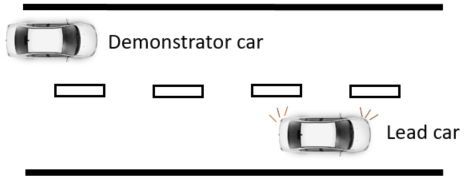
\includegraphics[scale=.6]{example12.png}
	\caption{In highway drone data, the \emph{indicator light} of the lead car would be missing, introducing a \emph{hidden common cause} between acceleration of demonstrator car and lane changing behavior of the lead car. }\label{fig:example1}
\end{figure}
%\end{wrapfigure}
%\todo{can we write demonstrator *car* and maybe also lead car or some other name for the other car?}


%\paragraph{Example of highway drone data:}
\begin{example}[Highway drone data]
\label{expl:i}
%In the development of self-driving cars, recently drones have been deployed to fly over highways and record the behavior of human-driven cars \cite{highDdataset}.
In the development of self-driving cars, recently drones have been deployed to fly over highways and record the behavior of human-driven cars \cite{highDdataset,zhan2019interaction}.
%This is a cheap way to collect large amounts of relevant data.
%But
Clearly, in such drone recordings, some crucial variables are either \emph{more noisy} than %a human or a sensor can observe
observed from within the car, or completely \emph{missing}, such as \emph{indicator lights}.
%

Assume we want to use such data %highway drone (where indicator lights are missing),
to learn, say, how an acceleration action $A$ of a ``demonstrator car'' affects the lane changing behavior $Z$ of a ``lead car'' in front of it on the slower lane, as depicted in Figure \ref{fig:example1}.
Slightly simplifying reality, assume the indicator light of the lead car serves as a perfect coordination device: it is on if and only if, subsequently, (1) the demonstrator car decelerates and (2) the lead car changes lane to the fast lane.
Now assume we just use the variables recorded in the drone data, where the indicator light is not contained, estimate $P(Z|A)$ from it, and naively consider it as the \emph{causal effect of $A$ on $Z$}. %\emph{causal effect of acceleration action $A$ on lane changing behavior $Z$}

This leads us to the conclusion that an agent in the place of the demonstrator can arbitrarily chose any acceleration or deceleration action as $A$, and the lead car will perfectly adapt $Z$ and only change lane when agent decelerates -- which in practice can lead to crashes. In the language of causal models \cite{pearl2009causality,spirtes2000causation}, the indicator light is a \emph{hidden common cause (confounder)}.
\end{example}












\paragraph{Main tasks, approach and contributions:}
In this paper, we address learning from demonstrations (LfD) under \emph{sensor-shift}, i.e., when %(a) the sensors of the demonstrator, (b) the sensors that we use to observe the demonstrator, and (c) the sensors of the AI agent we train differ. %completely or partially differ.
there are differences between (a)  the demonstrator's own sensory input, (b) our sensors that observe the demonstrator and (c) the sensory input of the agent we train.
Specifically, we consider two closely related ``subtasks'' of LfD: (1) inferring the effect of the demonstrator's decisions (as in Example \ref{expl:i}) and (2) imitating the demonstrator.
%
% which allows us to reason about (1) how the underlying \emph{mechanisms}, such as the influence of actions on the environment, are related to our observations, (2) to what extent these mechanisms are \emph{identifiable} from our observations, and (3) which mechanisms are \emph{invariant} between demonstration and target environment.

Our approach is based on causal models \cite{pearl2009causality,spirtes2000causation,peters2017elements}, which allow us to generalize from data beyond i.i.d.\ settings.
The idea is that, while some modular causal mechanisms that govern the data vary (the sensors), other mechanisms are \emph{invariant} (e.g., the action-effect). % and only some differ (the sensors).

Our main contributions are: %, for both subtasks:
\begin{itemize}

\item We rigorously analyze, on the population-level, %Proposition \ref{thm:lin}),
to what extent the relevant underlying mechanisms (the action-effect and the demonstrator policy) can be \emph{identified} and transferred from the available observations together with prior knowledge of sensor characteristics (Sections \ref{sec:general}, \ref{sec:deex}, \ref{sec:deexlin} and \ref{sec:imex}). And we propose algorithms to calculate them (Algorithms \ref{alg:gen} and \ref{alg:lin}). %We  to analyze to what extent mechanisms can be transferred.


%to what extent the relevant underlying mechanisms (the action-effect and the demonstrator policy) can be \emph{identified} and transferred from the available observations (Sections \ref{sec:general}, \ref{sec:deex}, \ref{sec:deexlin} and \ref{sec:imex}). And we propose algorithms to calculate them (Algorithms \ref{alg:gen} and \ref{alg:lin}). %We  to analyze to what extent mechanisms can be transferred.
\item We introduce several \emph{proxy methods} (Sections~\ref{sec:deav} and \ref{sec:imav}) which are easier to calculate, estimate from finite data and interpret than the exact solutions, alongside theoretical bounds on their closeness to the exact ones %(Sections~\ref{sec:deav}
(Propositions~\ref{thm:weightedproxy}, \ref{pro:imi2} and \ref{pro:imi5}). (Proofs are in the supplement\footnote{The supplement can be found at ``\url{https://doi.org/10.5281/zenodo.3549981}''.} of this paper.) %\citep{suppl}.)
%\item For each task, we propose several estimators of the relevant parameters. We propose both, exact solution ....... but also several proxies which are easier to easier to calculate and have a lower variance in the experiments.
\item We conduct \emph{experiments} to validate our two main methods on \emph{simulated and semi-real world} highway drone data used for autonomous driving (Section \ref{sec:exp}).

\end{itemize}



%
%
%\todo{OLD:}
%
%
%Running example of highway drone for autonomous driving:
%Recently, a rather cheap method for recording large amounts of data for these tasks has become popular: highways recorded from the bird view by a flying drone or by a camera mounted on some high spot \cite{}. It is clear that this data does contain information relevant for, say, imitation and decision-effect learning tasks for highly autonomous driving. However, crucial observations -- that are available to a car in the target environment -- are missing or more noisy than the target sensor: for instance, the blinker (indicator of direction) is not recorded. ............. For an illustration see Figure \ref{fig:example1}.
%\todo{blinker missing ...}
%
%
%\todo{OLD:}
%Consider the problem of having a demonstrator which we observe in order to imitate it or to learn the effects of its actions on the environment. The most well-studied version of this problem is where the source environment -- where the demonstrator acts and is recorded -- is equipped with the same sensors as the target environment -- where we, or the agent we design, act.
%However
%
%
%When learning from demonstrations, ideally one would like to also harness observations recorded by sensors different form those available in the target environment .
%
%%\todo{transfer}
%as much recorded demonstrations as possible, even when such demonstrations where recorded by sensors different from those cheap data as possible even when this data comes from
%
%
%\emph{sensors differ} between the source environment where demonstrations take place and the target environment where actions are taken.
%
%Even when the underlying dynamics etc. are the same, this poses a serious challenge and in the extreme case can make transfer impossible.
%
%sensor-shift
%sensor-variation
%sensor-
%
%
%
%
%\todo{OLD:}
%
%
%
%
%that the underlying \emph{(physical) mechanisms/laws/causal influence relations which are invariant} between the environments even though we have different sensors/representations. In particular for decision making it is clear that one needs the effetcs of actions, and not just their correlates.
%And to analyze the fundamental issue of to what extent these mechanisms can be \emph{identified} from the source environments sensor recordings.
%\todo{is it actually also hold for imitation in the sense of identifying the effect of the inputs of the demonstrator?}
%
%
%
%
%
%







\section{Related work}

%\todo{some is already in the Notes}
%
%
%
%
%
%
%
%\todo{The advantage of our work over other work that puts a higher priority on learning (e.g., \cite{stadie2017third}), is that our approach is more inspectable, principled and we can derive guarantees.}

\emph{Learning from demonstrations} (LfD) \cite{argall2009survey} is a broad area, with two concrete tasks being the ones we also consider in this paper: (1) inferring the effect of action on outcome given observation (we call it ``action-effect'' in our a-temporal framework, while in the language of \cite{argall2009survey} this is called the ``system model'' or ``world dynamics''), and (2) imitation learning (see next paragraph).
Generally in LfD, the problem that sensors differ between demonstrator, observer and target AI agent has been considered \cite{argall2009survey,ude2004programming,atkeson1997robot}.
In the language of \cite{argall2009survey}, this is described as the ``recording mapping'' or ``embodiment mapping'' not being the identity. However, we are not aware of any treatment of this problem which is as \emph{systematic and general} as ours in terms of  guarantees on exact and approximate identifiability. Instead, approaches are practically-focused, tailored to specific, say, robot tasks \cite{ude2004programming,atkeson1997robot}.


%\textbf{Causal inference} is the process of deducing cause-effect relationships among a set of variables \cite{pearl2009causality,peters2017elements}.
%There are different approach to discover such causal relationships. Some are based on pre-recorded observations \cite{louizos2017causal,maathuis2010predicting,lopez2017discovering,etesami2017econometric} and some are based on interventional data \cite{eberhardt2007interventions,tong2001active,shanmugam2015learning}.

%An important goal in both transfer learning and causal inference is to make accurate predictions when there exists differences between the source (the environment where the experiments are conducted) and the target domains.

%The key idea in transfer learning is that new experiments should transfer insights from previous experiments rather than starting learning anew \cite{saenko2010adapting,donahue2014decaf}.


Within LfD, \emph{imitation learning} means learning to perform a task from expert demonstrations \cite{ho2016generative,muller2006off}.
%In this task, the imitator (learner) is given only samples of trajectories from the expert (demonstrator). It is not allowed to query the expert for more data while training, and is not provided reinforcement signal of any kind.
There are two main approaches to address this problem: behavioral cloning \cite{pomerleau1991efficient}, which we are focusing on,
%which learns a policy as a supervised learning problem over state-action pairs from the demonstrator;
and inverse reinforcement learning (IRL) \cite{ng2000algorithms,ziebart2008maximum}. %, which finds a reward/cost function under which the demonstrator's behavior is explainable and reproducible.


%On the other hand, our proposed approach that lays more toward the behavior cloning -- because we do not specify a reward function -- %\footnote{This is in the sense that our learner imitates the demonstrator without specifying any reward function.}
%relaxes this setting.

The problem of bounding as well as transferring and integrating \emph{causal relations} across different domains has been studied by \cite{balke1994counterfactual,bareinboim2014generalizability,magliacane2017causal}. %\todo{maybe put balke1994counterfactual separately:
%This is also the case in the highway drone data example in Section \ref{sec:intro}.
%If the target environment is arbitrary, or drastically different from the study environment, no causal relations can be transferred to the the target environment
%Also \cite{} considers transfer between different domains/contexts.
But all this work does not consider the training of AI agents.
Within causal modelling, maybe closest related to our paper are \cite{bareinboim2015bandits,forney2017counterfactual,zhang2017transfer,geiger2016experimental}, who also study the integration of data from heterogeneous settings for training agents (often with latent confounders and from a multi-armed bandit perspective).

%Within causal modelling, maybe closest related to our paper are \cite{bareinboim2015bandits,forney2017counterfactual,zhang2017transfer}, who also study the integration of data from heterogeneous settings with latent confounders for training agents (from a multi-armed bandit perspective).
%\todo{OLD: }
%For example, \cite{zhang2017transfer} tackle the problem of transferring knowledge across bandit agents in settings where causal effects cannot be identified by standard learning techniques. Their approach consists of two steps: deriving bounds over the arms distribution and incorporating these bounds to search for more promising actions.
%However, they do neither consider identifiability \emph{up to a set} (as we do in Section \ref{sec:general}), nor continuous actions, which are highly relevant in practice (as we do in Sections \ref{sec:general}, \ref{sec:imitask} and \ref{sec:dea}), nor do they consider approximate identification (as we do in Sections \ref{sec:imitask} and \ref{sec:dea}).
%
%\todo{NEW: }
For example, \cite{zhang2017transfer} tackle the problem of transferring knowledge across bandit agents in settings where causal effects cannot be identified by standard learning techniques. Their approach consists of two steps: (1) deriving bounds over the effects of selecting arms and (2) incorporating these bounds to search for more promising actions.
However, when bounding the causal effect, they focus on binary variables, while we consider arbitrary finite as well as continuous ranges (which are highly relevant in practice) and they do not focus on general sensor-shifts.
%Moreover, they do not consider approximate identification (as we do in Sections \ref{sec:imitask} and \ref{sec:dea}).

The authors of \cite{causalconfusion} study ``causal confusion" in causal-model-free imitation learning. There, additional observations can lead to worse performance due to the mechanism (policy) that generates them differing between demonstrations and target environment.
However, in their model they assume that both the demonstrator and the imitator have (at least) the same observations.
This is not always the case, and therefore our treatment allows the observations to differ.




\begin{figure*}[t]
	\centering
	\begin{tikzpicture}[scale=1]
	\node at (3, 0) (A) {$A$};
	\node[var] at (4.5, 0) (R) {$\Out$};
	\node[hid] at (0, 0) (X) {$X$};
	\node[var] at (-1.5, -1.3) (Ws) {$\Obs_S$};
	\node[hid] at (1.5, -1.2) (Wd) {$\Obs_D$};

	\draw[->] (A) to (R);
	\draw[->] (X) to (Wd);
	\draw[->] (X) to (Ws);
	\draw[->] (Wd) to node [above,midway] {$\pi_D$} (A);
	\draw[->,bend left=40]  (X) to (R);
	\end{tikzpicture}
	\begin{tikzpicture}[scale=1]
	\node at (3, 0) (A) {$A$};
	\node[var] at (4.5, 0) (R) {$\Out$};
	\node[hid] at (0, 0) (X) {$X$};
	\node[var] at (1.5, -1.3) (Wt) {$\Obs_T$};

	\draw[->] (A) to (R);
	\draw[->] (X) to (Wt);
	\draw[->] (Wt) to node [above,midway] {$\pi_T$} (A);
	\draw[->,bend left=40]  (X) to (R);


	\node[var] at (-1.5, 0) (Ws) {$\phantom{\Obs_S}$};
	\end{tikzpicture}
	\caption{Causal DAGs. \textbf{Left:} source domain. \textbf{Right:} target domain. Circle means hidden to us.} % \todo{maybe put policies $\pi$ as squares}}
	\label{fig:cdag}
\end{figure*}

\section{Background}
\label{sec:background}

\paragraph{Conventions:}
We use $D(\cdot||\cdot)$, $H(\cdot)$, and $I(\cdot;\cdot|\cdot)$ to denote the Kullback-Leibler (KL) divergence, entropy, and mutual information, respectively \cite{cover2012elements}.
We consider both, discrete and continuous random variables; $\SumInt$ stands for the sum or integral, accordingly; $P(W)$ for the distribution of a variable $W$, and $p(w)$ for the density at value $W=w$. %, and will mention explicitly whenever we restrict to either case.
If not stated otherwise, we assume that distributions have full support\footnote{Full support is a commonly made \cite{pearl2009causality} but non-trivial assumption, important for identifiability.} and densities.


\newcommand{\PA}{\mathit{PA}}
\paragraph{Causal models:}
According to Pearl's definition \cite{pearl2009causality}, a \defi{causal model} is an ordered triple $(U, V, E)$, where $U$ denotes a set of \emph{exogenous variables} whose values are determined by factors outside the model (not observable); $V$ is a set of \emph{endogenous variables} whose values are determined within the model; and $E$ is a set of \emph{structural equations} that express, for each endogenous variable $W \in V$, the \emph{mechanism} of how $W$ is generated by certain other endogenous and exogenous variables. Namely, for all $W\in V$, we have
$$
W = f_W(\PA_W, U_W),
$$
 where $f_W(\cdot,\cdot)$ is a function and $\PA_W$ denotes the \defi{parent set} of variable $W$. $W$ is called a \emph{child} of $\PA_W$.
This induces a joint distribution over the endogenous variables, which can be factorized as follows:
$$
P(V) = \prod_{W \in V} P(W|\PA_W).
$$
This factorization is usually expressed using a \defi{directed acyclic graph (DAG)}, in which nodes represent the endogenous variables and arrows are from parents to their children.
It is also possible that a sub-set of $V$ is hidden. In this case, we denote the hidden variable with circles in the DAG.

The \defi{post-interventional distribution} is defined by replacing a subset of structural equations without generating cycles in the DAG \cite{pearl2009causality}. More specifically, the post-intervention distribution after (\textit{atomic}) intervening on variable $W$ is defined by replacing $f_W(\PA_W, U_W)$ with value $w$ and it is denoted by
$
P\big(V| do(W = w)\big).
$


%\paragraph{Causal models:}
%According to Pearl's definition \cite{pearl2009causality}, a \defi{causal model} is an ordered triple $(U, V, E)$, where $U$ denotes a set of exogenous variables whose values are determined by factors outside the model (not observable); $V$ is a set of endogenous variables whose values are determined within the model; and $E$ is a set of structural equations that express, for each endogenous variable $v_i \in V$, the \emph{mechanism} of how $v_i$ is generated by certain other endogenous and exogenous variables. Namely, for $v_i\in V$, we have $v_i = E_i(\pa(v_i), u_i)$, where $E_i(\cdot,\cdot)$ is a function and $\pa(v_i)$ denotes the \defi{parent set} of variable $v_i$. $v_i$ is called a child from $\pa(v_i)$.
%This induces a joint distribution over the endogenous variables, which can be factorized as follows:
%$
%P(V) = \prod_i P(v_i|\pa(v_i)).
%$
%This factorization is usually expressed using a \defi{directed acyclic graph (DAG)}, in which nodes represent the endogenous variables and there are arrows from parents to their children.
%It is also possible that a sub-set of $V$ is hidden. In this case, we denote the hidden variable with circles in the DAG.
%
%The \defi{post-intervention distribution} is define by replacing a subset of structural equations without generating cycles in the DAG. More specifically, the post-intervention distribution after intervening on variable $v_j$ is defined by replacing function $E_j(\pa(v_j), u_j)$ by function $\hat{E}_j(\hat{\pa}(v_j), \hat{u}_j)$ in the structural equations\footnote{A common type of intervention is \textit{surgical} intervention in which $\hat{E}_j(\hat{\pa}(v_j), \hat{u}_j)$ is simply a constant \cite{pearl2009causality}. } and it is denoted by
%$
%P\Big(V| do\big(v_j=\hat{E}_j(\hat{\pa}(v_j), \hat{u}_j)\big)\Big).
%$






\section{Setting and problem formulation}

\subsection{General model of our setting}
\label{sec:model}




\paragraph{Causal models of source and target domain.} There are two domains, the \emph{source domain} where the \emph{demonstrator (agent)} observes and acts, and the \emph{target domain} where the \emph{target agent}, which we design, observes and acts.
(By domain we mean the complete causal model of environment, sensors, and agent.)
The two domains, including what is hidden and what is observed by us, are depicted by the two causal DAGs in Figure \ref{fig:cdag} over the following variables:
$X$ is the \emph{state} of the system,
$A$ is the \emph{action} of the agent,
$Z$ stands for the \emph{outcome} (an abstract variable that could be, as in Example \ref{expl:i}, the state of cars in the the next time instance). %given state and action).
Regarding \emph{observations}, we assume that in the source domain we have
$Y_D$, the \emph{demonstrator's input}, generated by the demonstrator's sensors,
$Y_S$, the \emph{spectator's -- i.e., our -- observation} of the state of the source system,
and in the target domain we have
$Y_T$, the \emph{input to the target agent} from the target agent's sensors.
We often denote distributions over variables (e.g. $P(Z)$) in the source and target domain by subscript $S$ and $T$, respectively (e.g., $P_S(Z)$ and $P_T(Z)$).
Let $\pi_D(A|Y_D)$ denote the \emph{policy of the demonstrator},
and  $\pi_T(A|Y_T)$ denote the \emph{policy of the target agent}.

\paragraph{Relationship between source and target domain, and what is known to us.}
We assume that the two domains are related by sharing the same invariant mechanism for outcome given state and action, i.e.,
\begin{align*}
P_T(\Out|A, X)=P_S(\Out|A, X),
\end{align*}
so that we can drop the subscript and just write $P(\Out|A,X)$.
%
%\paragraph{What is known to us:}
%\todo{maybe also put part of the above paragraph here}
We assume we are given $P_S(\Out, A, \Obs_S)$ (or a sample of it), as well as the sensor characteristics\footnote{This may be based on performing an experimental system identification of the sensors or using physical knowledge.} $P_S(Y_S|X)$ and $P_T(Y_T|X)$.
%in an experimental setup where we controlled the state $X$, or that we know some properties a priori.}



\subsection{Problem formulation}
\label{sec:problem}


The overarching goal is to design the target agent that observes and successfully acts in the target domain, based on what we know from the source domain and its relation to the target domain.
%Recall that (Section \ref{sec:model}) from the source domain we know $P_S(Z, A, Y_S)$ (or a sample of it).
We consider two specific tasks that serve this overarching goal:
\begin{task}[\Dec]
	\label{task:d}
	Infer $P_T(\Out|\dob{A}, Y_T)$, the effect of action $A$ on outcome $Z$ conditional on observation $Y_T$ in the target domain.%
	\footnote{Once the effect $P_T(\Out|Y_T, \dob{A})$ is inferred, what remains to be done for designing the target agent is to fix a utility function $u(\Out)$ on the outcome, and then pick the optimal $a$ by, say, maximizing $\E_T(u(\Out)|\dob{a}, y_T)$ w.r.t.\ $a$.}
\end{task}
\begin{task}[Imitation transfer learning task]
\label{task:i}
Learn a policy $\pi_T(A|\Obs_T)$ for the target agent (also called \defi{imitator} in this task) %, i.e., a conditional distribution over the actions given the observation $\Obs_T$,
such that it behaves as similarly as possible to the demonstrator %in the source domain
(details follow).
%\todo{OLD:}
%Infer the target agent's policy $\pi_T(A|\Obs_T)$, i.e., a conditional distribution over the actions given the observation $\Obs_T$ in the target domain, such that the target agent (also called \defi{imitator} in this task) behaves similar to the demonstrator in the source domain.
\end{task}





\section{Basic step addressing both tasks: equations and algorithm}
\label{sec:general}

In this section, we make general derivations about our model (Section \ref{sec:model}), which serve as steps towards \emph{both}, the imitation and the action-effect transfer learning tasks.
% (Task~\ref{task:d} and \ref{task:i}).

%Under a given policy $\pi$, we have \todo{what about dropping superscript $\pi_T$ here?}
%\begin{align}\label{eq:T1}
%&P^\pi_T(\Out, \Obs_T, A)=P_T(\Out|A, \Obs_T)\pi(A|\Obs_T)P_T(\Obs_T),  \\ \label{eq:S1}
%&P_S(\Out, \Obs_S, A)=\sum_{\obs_D}P_S(\Out, \Obs_S, \obs_D, A)=\sum_{\obs_D}P_S(\Out|A, \obs_D, \Obs_S)\pi_D(A|\obs_D)P_S(\obs_D, \Obs_S),
%\end{align}

%where $\pi$ and $\pi_D$ denote the policy in the source domain and the policy of the demonstrator, respectively.
%\begin{assumption}
%	We assume that both domains have the same dynamic that is $P_T(\Out|A, X)=P_S(\Out|A, X)=P(\Out|A,X)$.
%	But: varying: senors/measurement device.
%\end{assumption}



\paragraph{Basic equation:}
Our model (Section \ref{sec:model}) implies the following equations, for all $\out, a, \obs$:

\begin{align}%\notag
&p_S(\out, a, \obs_S)  = \SumInt_x p_S(\obs_S|x) p_S(z, a, x)  \label{eqn:gen1} \\
&= \SumInt_{x, y_D} p_S(\obs_S|x) p(\out | a, x) \pi_D(a|\obs_D) p_S(\obs_D, x). \label{eqn:gen}
\end{align}
%
%\vmin
%Eq.~\ref{eqn:gen}
%HEAD
%These are the basic equations that relates what is known -- $p_S(\out, a, \obs_S)$ (l.h.s. of Eq.~\ref{eqn:gen1} \todo{uniformify equation references .... (...) (instead of Eq. (...)) everywhere?} ) -- to what we would like to know (r.h.s.\ of Eq.~\ref{eqn:gen}): $\pi_S(a|\obs_D)$ for Task \ref{task:i} and $p(\out | a, x)$ for Task \ref{task:d}.
%=======
These are the basic equations that relates what is known -- $p_S(\out, a, \obs_S)$ (l.h.s. of~\eqref{eqn:gen1}) -- to what we would like to know (r.h.s.\ of~\eqref{eqn:gen}): $\pi_D(a|\obs_D)$ for Task \ref{task:i} and $p(\out | a, x)$ for Task \ref{task:d}.
%>>>>>>> ee5be1916be43211d895dc0edf5e4d0c6ff6eb6d
More specifically, these equations \emph{constrain} the unknown quantities to a set of possibilities.
This is exactly the set up to which we can \emph{identify} \cite{pearl2009causality} them. % unknown quantities.

%Let us first write down a very basic equation that relates the known with what we want to know and serves as a basis for various more specific tasks in the subsequent sections.
%Based on the causal DAG and usual probability calculus, the unknowns are constraint to a ``possibilities set'' -- denoted by %$\pos$
%-- by the knowns together with the following equation system:
%We have
%\begin{align}
%p_S(\out, a, \obs_S)  = \SumInt_x p(\obs|x) p(x, a, \obs) = \SumInt_x p(\obs|x) p(\out | a, x) \pi_S(a|\obs_D) p(\obs_D, x), \text{ for all $\out, a, \obs$}. \label{eqn:gen}
%\end{align}
%aa


\newcommand{\w}{P(\out, a, X)}
\newcommand{\F}{[P( y^i | x^j)]_{i,j=1}^{m, \ell}}
\newcommand{\vv}{P(\out, a, Y_S)}


\paragraph{Finite linear equation system in discrete case:}
Solving %the first part of
~\eqref{eqn:gen1} for $p_S(z, a, x)$ is an important intermediate step to addresses Task~\ref{task:d} and \ref{task:i} simultaneously, since $p_S(z, a, x)$ contains all the information that $p_S(z, a, \obs_S)$ contains about $\pi_D(a|y_D)$ and $p(\out | a, y_T)$.
(In particular, in the classical case of $Y_S=Y_T=Y_D=X$, $p_S(z, a, x)$ uniquely determines the latter two quantities via marginalization/conditioning.)
%      ... that .. has and
%in the important case of $Y_S=Y_T=Y_D=X$, .... simple marginalization/ conditioning gives us the unique solution ....addresses both tasks simultaneously, since $\pi_S(a|x)$ and $p(\out | a, x)$ are determined by $p_S(x, a, \obs_S)$.
So let us for a moment focus on~\eqref{eqn:gen1}.
In the discrete case, it can be rewritten as the following collection of matrix equations.
%\todo{ALTERNATIVE FOMRULATION:}
Let  $\{ x^1, \ldots, x^\ell \}$ and $\{ y^1, \ldots, y^m \}$ be the range of $X$ and $\Obs_S$, respectively.
Then, for all $ \out, a$,
	\begin{align}
	\underbrace{\left[ \!\!\!\begin{array}{c} P(\out, a, \obs^1) \\ \vdots \\ P(\out, a, \obs^m) \end{array} \!\!\right]}_{\vv \in \mathbb{R}^{m}} \!\!\!=\!\!\!
	\underbrace{\left[ \!\!\!\begin{array}{cc} P( y^1 | x^1) \cdots\!\!\!\!\!\! \!\!  & P( y^1 | x^\ell) \\ \vdots & \vdots \\   P( y^m | x^1)  \cdots\!\!\!\!\!\! \!\!  & P( y^m | x^\ell) \end{array}\!\!\! \right]}_{\F \in \mathbb{R}^{  m \times \ell} } \!
	\underbrace{\left[ \!\!\!\begin{array}{c} P(\out, a, x^1) \\ \vdots \\ P(\out, a, x^\ell) \end{array} \!\!\!\right]}_{P(\out, a, X)  \in \mathbb{R}^{\ell}} \!\!. \label{eqn:possible}
	\end{align}
%
%
%\newcommand{\pos}{\mathit{Possib}}
%We know the vectors $P_{\Out, A, \Obs_S} \in \mathbb{R}^{\rngs{\Out} \rngs{\Obs_S} \rngs{A}}, P(\Obs_S | X) \in \mathbb{R}^{\rngs{\Obs_S}  \rngs{X}}$.
%\todo{ALTERNATIVE FOMRULATION:}
%Let $\bar{P}(\out, a, \Obs_S) = [ P(\out, a, \obs^1) \ \cdots \ P(\out, a, \obs^m)]^T$
%\todo{ALTERNATIVE FOMRULATION:}
%\begin{small}
%\begin{align}
%\left[ \!\!\!\begin{array}{c} P(\out, a, \obs^1) \\ \vdots \\ P(\out, a, \obs^m) \end{array} \!\!\right] \!\!=\!\!
%\left[ \!\!\!\begin{array}{cc} P( y^1 | x^1) \cdots\!\!\!\!\!\! \!\!  & P( y^1 | x^\ell) \\ \vdots & \vdots \\   P( y^m | x^1)  \cdots\!\!\!\!\!\! \!\!  & P( y^m | x^\ell) \end{array}\!\!\! \right] \!\!\!
%\left[ \!\!\!\begin{array}{c} P(\out, a, x^1) \\ \vdots \\ P(\out, a, x^\ell) \end{array} \!\!\!\right] , \label{eqn:possible}
%\end{align}
%\end{small}
%
%
%\todo{ALTERNATIVE FOMRULATION:}
%\begin{small}
%	\begin{align}
%	\left[ \! \begin{array}{c} P(\out, a, \obs^1) \\ \vdots \\ P(\out, a, \obs^m) \end{array} \!\right] =
%\left[\! \begin{array}{cc} P( y^1 | x^1) & \cdots  \\ \vdots &   \\   P( y^m | x^1) & \cdots  \end{array} \!\right]
%	\left[\! \begin{array}{c} P(\out, a, x^1) \\ \vdots \\ P(\out, a, x^\ell) \end{array} \!\right] , \label{eqn:possible}
%	\end{align}
%\end{small}
%
%
%
%\todo{ALTERNATIVE FOMRULATION:}
%\begin{small}
%\begin{align}
%\left[ \! \begin{array}{c} P(\out, a, \obs^1) \\ \vdots \\ P(\out, a, \obs^m) \end{array} \!\right] =
%\F
%\left[\! \begin{array}{c} P(\out, a, x^1) \\ \vdots \\ P(\out, a, x^\ell) \end{array} \!\right] , \label{eqn:possible}
%\end{align}
%\end{small}
%\todo{OLD:}
%Let  $\{ x^1, \ldots, x^\ell \}$ and $\{ y^1, \ldots, y^m \}$ be the range of $X$ and $\Obs_S$, respectively,
%Then, for all $ \out, a$, $[ P(\out, a, \obs^1) \ \cdots \ P(\out, a, \obs^m)]^T$ is
%%\begin{small}
%%\begin{align}\notag
%%&\left[ \begin{array}{c} P(\out, a, \obs^1) \\ \vdots \\ P(\out, a, \obs^m) \end{array} \right] = \\
%%&\left[ \begin{array}{ccc} P( y^1 | x^1) & \cdots & P( y^1 | x^\ell) \\ \vdots & & \vdots \\   P( y^m | x^1) & \cdots & P( y^m | x^\ell) \end{array} \right]
%%\left[ \begin{array}{c} P(\out, a, x^1) \\ \vdots \\ P(\out, a, x^\ell) \end{array} \right] , \label{eqn:possible}
%%\end{align}
%%\end{small}
%\begin{small}
%\begin{align}
%%\left[ \!\!\begin{array}{c} P(\out, a, \obs^1) \\ \vdots \\ P(\out, a, \obs^m) \end{array} \right] =
%\left[ \begin{array}{ccc} P( y^1 | x^1) & \cdots & P( y^1 | x^\ell) \\ \vdots & & \vdots \\   P( y^m | x^1) & \cdots & P( y^m | x^\ell) \end{array} \right]
%\left[ \begin{array}{c} P(\out, a, x^1) \\ \vdots \\ P(\out, a, x^\ell) \end{array} \right] , \label{eqn:possible}
%\end{align}
%\end{small}
%\todo{Proposal for general algorithm paragraph: either complete Algorithm 1 to an algo which solves (2) (similar to what was in the Notes for the imitation part) or add an Algo which solves (2) by calling Algo 1 as subrutine and then does the remaining constraint satisfaction stuff etc. (reason: otherwise it's too detached from what the papere is about, in particular at this early stage) Furthermore: need to replace x, A, y, etc. by other symbols -- collision}

\paragraph{Algorithm for solution set in discrete case:}
Algorithm \ref{alg:gen} yields a parametrization of the set of all possible solutions $P(\out, a, X) \in \mathbb{R}^\ell$ to~\eqref{eqn:possible}, for any $\out, a$. Specifically, it outputs the finite set of \emph{corner vectors} whose \emph{convex combinations parametrize} \emph{the solution set}.

It uses singular-value decomposition (SVD) to cope with non-invertibility, and then a routine inspired by the simplex algorithm to account for the constraint that the output has to be a proper probability distributions.\footnote{Since the left hand side of \eqref{eqn:possible} is a probability vector, it is not necessary to bound $P(z, a, x^i)$ by one.}

For the algorithm, w.l.o.g., we assume $m \leq \ell$ and that $\F$ has full rank (otherwise one removes linearly dependent rows).
Note that if $m=\ell$ and $\F$ is non-singular, then %$\vv=\F \cdot \w$
%HEAD
\eqref{eqn:possible} determines $\w$ uniquely, via a simple matrix inversion.
Therefore, for this algorithm, the interesting scenario is % is The interesting scenario where our algorithm applies is when
	$m<\ell$. This is the case, e.g., in Example \ref{expl:i} -- the highway drone data where indicator lights are not recorded.
%=======
%\eqref{eqn:possible} determines $\w$ uniquely, via a simple matrix inversion.
%Therefore, for this algorithm, the interesting scenario is % is The interesting scenario where our algorithm applies is when
%	$m<\ell$. This is the case, e.g., in Example \ref{expl:i} -- the highway drone data where indicator lights are not recorded.
%>>>>>>> ee5be1916be43211d895dc0edf5e4d0c6ff6eb6d
% is missing as in Example \ref{expl:i}.
%This can occur when for example, the demonstrator observes the speed and the indicator of the surrounding vehicles but the imitator's observation from the demonstrator contains only the speed.


%\todo{maybe put the SVD-based algo here as a subroutine/module which can be used by many of the other algorithms? or put the more complete algorithm that solves the above eq. including constraints etc.?}
%Let us now introduce an algorithm that finds the solution set of Eq.~\ref{eqn:possible}.
%It is heavily based on finding the solution set of a system of linear equations of the form $v=F w$ (similar to \eqref{eqn:possible}), where $v\in\mathbb{R}^m$, $w\in\mathbb{R}^\ell$, and $F\in \mathbb{R}^{m\times\ell}$.
%%In this section, we introduce an algorithm for finding the solution set of a system of linear equations of the form $x=Ay$ (similar to \eqref{eqn:possible}), where $x\in\mathbb{R}^m$, $y\in\mathbb{R}^\ell$, and $A\in \mathbb{R}^{m\times\ell}$.
%If $m=\ell$ and $\F$ is non-singular, then $\vv=\F \w$ determines $\w$, uniquely.
%The interesting scenario is when $m<\ell$. This can occur when for example, the demonstrator observes the speed and the indicator of the surrounding vehicles but the imitator's observation from the demonstrator contains only the speed.
%In this case, assume that $F$ is full rank. Algorithm \ref{alg:svd} summarizes the steps\footnote{Since the left hand side of \eqref{eqn:possible} is a probability vector, it is not necessary to bound $P(z, a, x^i)$ by one.} for finding the solution set of $v=F w$.
% and without of loss of generality, let $F\in\mathbb{R}^{m\times m}$ which consists of the first $m$ columns of $A$ is non-singular.
%In this case, let $U^T\Sigma V$ denote the singular-value decomposition of $A$, then we have
%\begin{small}
%\begin{align}
%&y\in \left\{u: u=\sum_{i=1}^{\ell-m}\xi_i V \begin{bmatrix}
%    \textbf{0}  \\
%    e_i
%\end{bmatrix} + \begin{bmatrix}
%   F^{-1}x \\
%     \textbf{0}
%\end{bmatrix}\right\}
%\end{align}
%\end{small}
%where $e_i$ is a vector of length $\ell-m$ whose elements are zero except its $i$ entry.
\begin{algorithm}[t]
	\label{alg:gen}
	\caption{Finding solution set for \eqref{eqn:possible}}\label{alg:svd}
	\KwIn{$\vv$ (l.h.s.\ of \eqref{eqn:possible}), $\F$}
	\KwOut{$\zeta_1, \ldots, \zeta_k \in \mathbb{R}^{\ell}$, such that their convex hull is the solution set to  \eqref{eqn:possible}
%		\begin{small}$\forall v\in\{ \sum_i \lambda_i \zeta_i : 0 \leq \lambda_i \leq 1,$ $ \sum_i \lambda_i=1 \}$\end{small}, $M \cdot v+b$ is a solution to \eqref{eqn:possible}
	}
	Rearrange columns of $\F$ such that $\F=[D\ E]$ and $D \in \mathbb{R}^{m \times m}$ is non-singular\;
	$U\Sigma V^T\leftarrow$ SVD of $\F$   \;
	\For{$i=1$ \KwTo $\ell-m$}{$e_i\leftarrow$ zero vector of length $\ell-m$ whose $i$th entry is one\;}
	$M\leftarrow \small{V\begin{bmatrix} \textbf{0} & \!\!\!\!\!\cdots\!\!\!\!\! & \textbf{0}  \\
    e_1 & \!\!\!\!\!\cdots\!\!\!\!\! & e_{\ell-m} \end{bmatrix}}$,
	$b \leftarrow \begin{bmatrix}   D^{-1} \vv \\     \textbf{0}
\end{bmatrix}$\;
 $i \leftarrow 1$\;
	\For{any sub-matrix $R$ of $M$ with dimension $(\ell-m)\times(\ell-m)$}{$\hat{b}\leftarrow$  %the corresponding sub-vector of $b$ with length $\ell-m$  \todo{
			the sub-vector of $b$ of length $\ell-m$ that corresponds to the selected rows of $M$\;
	\If{$R^{-1}$ exists and $- M R^{-1}\hat{b}+b \geq 0$}{$\zeta_i\leftarrow -  M R^{-1}\hat{b}+b$\; $i \leftarrow i + 1$\;}
%	\todo{how exactly is it made sure that the $< 1$ constraint is met?}
%	\todo{OLD: } $\zeta_i\leftarrow R^{-1}\hat{b} \todo{(- \hat{b})}$, if $R^{-1}$ exists\;
%	If $M\zeta_i+b<0$ reject $\zeta_i$, otherwise $i \leftarrow i + 1$\;}
}
\end{algorithm}
%It is important to mention that the solution set of \eqref{eqn:possible} needs to satisfy another set of constrains that is $0\leq P(z, a, x^i)$ for $i=1,...,\ell$. This impose a set of constraints on $\{\xi_1,...,\xi_{m-\ell}\}$ in Algorithm \ref{alg:svd}.
%Depending on the application, it might be necessary that the solution of \eqref{eqn:possible} satisfies additional constraint or properties. For instance in the imitation learning task, we might want the safest or most comfortable driving policy that imitates the demonstrator. This can be formulated as a linear programming or convex optimization with a set of linear constraints such as \eqref{eqn:possible}.
%See experiment section.
%\todo{add Eq.~\ref{eqn:possible} solution Algorithm as superroutine}


%$w \leftarrow \sum_{i=1}^{\ell-m}\xi_i V \begin{bmatrix} \textbf{0}  \\
%    e_i \end{bmatrix} + \begin{bmatrix}   D^{-1}x \\     \textbf{0}
%\end{bmatrix}$\;


%\section{Approach to imitation learning and \dec}





\section{Approach to the \dec}
\label{sec:dea}



%Let us now address Task~\ref{task:d} -- inferring the target domain's action-effect $P_T(\Out|\dob{A}, Y_T)$ (which could also be referred to as the target domain's ``dynamics'').
Let us now address Task~\ref{task:d} -- inferring the target domain's action-effect $P_T(\Out|\dob{A}, Y_T)$.
%several methods for several settings (discrete and continuous), yielding exactwill do this for discrete and continuous settings, and in an ex


\begin{example}
	To illustrate what can go wrong when naively addressing this task, let us get back to the highway drone data (Example \ref{expl:i}). There, in the source domain, the indicator light is not observed by us, and for simplicity we assumed that there are no other variables, i.e., $Y_S$ is empty/constant. Our informal argument in that example can now be stated formally based on causal models (Section \ref{sec:background}):
	Observe that in the causal DAG (Figure \ref{fig:cdag}), $X, Y_D$ are \emph{hidden confounders} that introduce ``spurious correlations'' between $A$ and $Z$. Therefore, in the generic case, the naive guess $P_S(\Out|a)$ does not coincide with the actual action-effect $P_S(\Out|\dob{A})$ ($= P_T(\Out|\dob{A})$).
\end{example}

%\begin{goal}
%	Infer $P_T(\Out|Y_T, A)$ (as intermediate step towards the end goal of picking the optimal policy $\pi_T(A | \Obs_T)$).
%\end{goal}


\begin{assumption}
	\label{asm:d}
	In this section, we assume the target agent observes the full state, i.e., $Y_T{=}X$.\footnote{Observability of $X$, similar as in Markov decision processes (MDPs), seems to be a good approximation to many real-world situations while at the same time keeping the analysis instructive. We make no assumption w.r.t.\ $Y_D$.}
	%This implies that the action-effect $P_T(\Out|\dob{A}, Y_T)$ coincides with $P_T(\Out|A, Y_T)$ ..........  So in this section, the quantity we want to infer is .........
	%W.l.og. we assume that $Y_S = f_{Y_S}(X)$, i.e., a deterministic relationship (this is, when just considering the general model, w.l.og., because if there was additional noise $N$, i.e. $Y_S = f_{Y_S}(X, N)$, we can just incorporate it into $X$, i.e., ``$X := (X, N)$''!)
	%\todo{PROBLEM: but then $Y_T = X$ doesn't make sense anymore.}
\end{assumption}

%Observe that
Under Assumption \ref{asm:d}, we have
$$
P_T(\Out|\dob{A}, Y_T) = P_T(\Out|\dob{A}, X) = P(\Out|A, X).
$$
 So Task~\ref{task:d} means inferring $P(\Out|A, X)$  (which could also be referred to as the (target domain's) ``dynamics'').
We now propose three methods, which differ w.r.t.\ the setting in which they are applicable and/or w.r.t.\ yielding exact or approximate solutions.





\subsection{Exact solution set in the discrete case}
\label{sec:deex}

In the case of all variables being discrete, we can build on our basic step in Section \ref{sec:general} to analytically find the set of possible action-effects $P(\Out|X, A)$ as follows: first we deploy Algorithm \ref{alg:gen} to get all possible $P(\Out,X, A)$, and then from this (simply by dividing by the marginals), we get  $P(\Out|X, A)$.




\subsection{Exact solution in the linear invertible continuous case}
\label{sec:deexlin}


In the continuous case, the general identification analysis -- the analysis of the solution set of \eqref{eqn:gen} -- is very difficult because the vectors space is infinite-dimensional.
Therefore let us here consider the special case of \emph{linear} relationships.


%\subsubsection{Continuous case -- linear special case -- population-level equation and sample-level algorithm}

\newcommand{\Oa}{W}
\newcommand{\oa}{w}
\newcommand{\om}{F}
\newcommand{\No}{N}
\newcommand{\no}{n}
\newcommand{\Noz}{O}
\newcommand{\noz}{o}

\newcommand{\stax}{\left[\begin{smallmatrix}A \\ X\end{smallmatrix}\right]}

\newcommand{\samplelen}{\ell}

\newcommand{\idm}{\mathbf{1}}
%For ease of notation, let $\Oa$ the stacking of $A$ and $Z$, i.e., .


\begin{assumption}
	\label{eqn:contas}
	In this Section \ref{sec:deexlin}, assume all relationships are linear, in particular, for matrices $D, E, F$,
	%
	%\noindent
	%\begin{tabularx}{\linewidth}{XXX}
	%\begin{equation}
	%a = b \label{eqab}
	%\end{equation}
	%& \[ \text{and} \] &
	%\begin{equation}
	%c = d \label{eqcd}
	%\end{equation}
	%\end{tabularx}
	%\begin{small}
	\begin{align}
	\Obs_S &= \om X + \No ,\quad \label{eqn:c1} \\ %% \label{eqn:c1} ,\\
	\Out &= [D\ E] \left[
	\begin{array}{c}
	A \\ X
	\end{array}
	\right]
	+ \Noz \label{eqn:c2}
	%\label{eqn:c12}
	\end{align}
	%\end{small}
	with $\No, \Noz$ the usual noise terms that are independent of all other (non-descendant) variables.
\end{assumption}%
We propose Algorithm \ref{alg:lin} as (sample-level) method in this setting.



\begin{algorithm}[t]
	%\begin{minipage}[h]{.55\linewidth}
	%\begin{algorithmic}
	\label{alg:lin}
	\caption{Exact linear action-effect transfer method (sample-level)}
	\KwIn{sample $(\out_1, a_1, \obs_1), \ldots, (\out_\samplelen, a_\samplelen, \obs_\samplelen)$ from $P(\Out, A, Y_S)$; prior knowledge $F$, $\Sigma_{N N}$ (see \eqref{eqn:c1}); regularization parameter $\lambda$} %\\
	\KwOut{Estimates $\hat{D}, \hat{E}$ for the regression matrices $D, E$ (see \eqref{eqn:c2})}
	%\Begin{dsadas\\asd}
	%\State
	Calculate the empirical covariance matrices $\hat{\Sigma}_{Z A}, \hat{\Sigma}_{Z Y_S}, \hat{\Sigma}_{A Y_S}, \hat{\Sigma}_{Y_S Y_S}$ from the sample \label{line:s}\\
	Add a regularization term $\lambda \idm$ to $\hat{\Sigma}_{A A}$ and $\hat{\Sigma}_{Y_S Y_S}$\\
	%\State
	Calculate the Schur complements\newline
	%\begin{align*}
	$S_1 := \hat{\Sigma}_{A A} - \hat{\Sigma}_{A Y_S} (\Sigma_{Y_S Y_S} - \Sigma_{\No \No })^{-1} \hat{\Sigma}_{Y_S A}$, %\\
	$S_2 := \hat{\Sigma}_{Y_S Y_S} - \Sigma_{\No \No } - \hat{\Sigma}_{Y_S A} \hat{\Sigma}_{A A}^{-1} \hat{\Sigma}_{A Y_S}$.\\
	%\end{align*}
	%\State
	Calculate the estimates
	$\hat{D} := \hat{\Sigma}_{\Out A}  S_1^{-1} - \hat{\Sigma}_{\Out Y_S} (\hat{\Sigma}_{Y_S Y_S} - \Sigma_{\No \No })^{-1} \hat{\Sigma}_{Y_S A} S_1^{-1}$, and
	$\hat{E} := - \hat{\Sigma}_{\Out A} S_1^{-1} \hat{\Sigma}_{A Y_S} (\hat{\Sigma}_{Y_S Y_S} - \Sigma_{\No \No })^{-1} + \hat{\Sigma}_{\Out Y_S} S_2^{-1} ) F$
	%	Calculate basis to parametrize the solution space of Eq.\ \ref{eqn:possible} \todo{elaborate}\\
	%	From this, calculate parametrization of $P_{Z|X,A}$ \todo{elaborate}
\end{algorithm}
%
%
%%\begingroup
%%\setlength\intextsep{0pt}
%%
%%
%%\DecMargin{0.1cm}
%%
%%
%%
%\hfill % THIS IS IMPORTANT TO PLACE IT HERE
%%%removedVspace
%%
%%\newfloat{algorithm}{t}{lop}
%%
%%\begingroup
%%\setlength{\columnsep}{0pt}%
%\begin{wrapfigure}{r}{0.55\textwidth}
%	%%removedVspace
%	%
%	%\begin{figure}[h]
%	%\centering
%	%\begin{minipage}[h]{.55\linewidth}
%	%\raggedright
%	%\begin{wrapfigure}{htbp}{0.55\textwidth}
%	%\begin{floatingfigure}[r]{0.55\textwidth}
%	%%removedVspace
%	%\begin{figure}[htbp]
%	%\begin{minipage}[h]{.55\linewidth}
%	%\begin{algorithm}[H]
%	\begin{algorithm}[H]
%		%\begin{minipage}[h]{.55\linewidth}
%		%\begin{algorithmic}
%		\label{alg:lin}
%		\caption{Sample-level continuous linear invertible decision-effect learning}
%		\KwIn{sample $(\out_1, a_1, \obs_1), \ldots, (\out_\samplelen, a_\samplelen, \obs_\samplelen)$; prior knowledge $F$, $\Sigma_{N N}$ (see Eq.~\ref{eqn:c12})} %\\
%		\KwOut{Estimates $\hat{D}, \hat{E}$ for the regression matrices $D, E$ (see Eq.~\ref{eqn:c12})}
%		%\Begin{dsadas\\asd}
%		%\State
%		Calculate the empirical covariance matrices $\hat{\Sigma}_{Z A}, \hat{\Sigma}_{Z Y}, \hat{\Sigma}_{A Y}, \hat{\Sigma}_{Y Y}$ from the sample \label{line:s} \\
%		%\State
%		Calculate the Schur complements
%		%\begin{align*}
%		$S_1 := \Sigma_{A A} - \Sigma_{A Y} (\Sigma_{Y Y} - \Sigma_{\No \No })^{-1} \Sigma_{Y A}$, %\\
%		$S_2 := \Sigma_{Y Y} - \Sigma_{\No \No } - \Sigma_{Y A} \Sigma_{A A}^{-1} \Sigma_{A Y}$.\\
%		%\end{align*}
%		%\State
%		Calculate the estimates
%		$\hat{D} := \Sigma_{\Out A}  S_1^{-1} - \Sigma_{\Out Y} (\Sigma_{Y Y} - \Sigma_{\No \No })^{-1} \Sigma_{Y A} S_1^{-1}$, and
%		$\hat{E} := - \Sigma_{\Out A} S_1^{-1} \Sigma_{A Y} (\Sigma_{Y Y} - \Sigma_{\No \No })^{-1} + \Sigma_{\Out Y} S_2^{-1} ) F$
%		%	Calculate basis to parametrize the solution space of Eq.\ \ref{eqn:possible} \todo{elaborate}\\
%		%	From this, calculate parametrization of $P_{Z|X,A}$ \todo{elaborate}
%	\end{algorithm}
%	%\end{algorithmic}
%	%\end{minipage}
%	%\end{algorithm}
%	%%removedVspace
%	%\end{wrapfigure}
%	%%\end{floatingfigure}
%	%\end{minipage}
%	%\end{figure}
%	%%removedVspace
%\end{wrapfigure}
%%
%%\endgroup
%%
%%
%%
%%We have
%%\begin{align}
%%\Sigma_{.........} &= \left[
%%\begin{array}{ccc}
%%\Sigma_{\Out \Out} & \Sigma_{\Out A} & \Sigma_{\Out \Obs} \\
%%\Sigma_{A \Out} & \Sigma_{A A} & \Sigma_{A \Obs} \\
%%\Sigma_{\Obs \Out} & \Sigma_{\Obs A} & \Sigma_{\Obs \Obs}
%%\end{array}
%%\right] \\
%%\Sigma_{\Oa \Obs} &=  \Sigma_{\Oa X}  \om^T \\
%%\Sigma_{\Obs \Obs} &=  \om \Sigma_{X X}  \om^T + \Sigma_{\No \No}
%%\label{eqn:cont}
%%\end{align}
%%
%%
%%%removedVspace
%%
%%
%%\endgroup
\begin{proposition} %[Soundness of Algorithm~\ref{alg:lin}]
	\label{thm:lin}
	Assume all variables have mean zero (otherwise center them).
	Furthermore, assume that $X$ and $Y_S$ have the same dimension, and that $F$ (in \eqref{eqn:c1}) is invertible.
	Then Algorithm~\ref{alg:lin} is \emph{sound} in the following sense: when replacing the empirical covariance matrices
	$$
	\hat{\Sigma}_{Z A}, \hat{\Sigma}_{Z Y_S}, \hat{\Sigma}_{A Y_S}, \hat{\Sigma}_{Y_S Y_S}
	$$
	 in Line~\ref{line:s} by their population-level counterparts, and setting the regularization term $\lambda=0$, the output will be the true $D, E$ (in \eqref{eqn:c2}).
	%The regression coefficients $(D, E)$ of $\Out$ conditioned on $A, X$ are given by:
	%\begin{align}
	%(D, E) &= \left( \Sigma_{\Out A}  S_1^{-1} - \Sigma_{\Out Y} (\Sigma_{Y Y} - \Sigma_{\No \No })^{-1} \Sigma_{Y A} S_1^{-1} \right. , \\
	%&\left. ( - \Sigma_{\Out A} S_1^{-1} \Sigma_{A Y} (\Sigma_{Y Y} - \Sigma_{\No \No })^{-1} + \Sigma_{\Out Y} S_2^{-1} ) F \right) ,
	%\end{align}
	%where, as usual, the Schur complements are defined as
	%\begin{align}
	%S_1 &:= \Sigma_{A A} - \Sigma_{A Y} (\Sigma_{Y Y} - \Sigma_{\No \No })^{-1} \Sigma_{Y A} \\
	%S_2 &:= \Sigma_{Y Y} - \Sigma_{\No \No } - \Sigma_{Y A} \Sigma_{A A}^{-1} \Sigma_{A Y} .
	%\end{align}
\end{proposition}%






\subsection{Average-based action-effect proxy in the general case}
\label{sec:deav}




%This is a generalization of the results in Section \ref{sec:proxy_s}.


The \emph{exact} general solution can be difficult to handle in terms of computation, estimation and analysis, and the linear case (Section \ref{sec:deexlin}) is of course restrictive.
Let us define the following \emph{average-based action-effect proxy} of the density $p(\out|x, a)$, for all $\out,x,a$, defined only based on things we do know (from the source domain):

\begin{align}
\tilde{p}(\out|x, a)\! :=\! \SumInt_{\obs_S} p_S(\out|\obs_S, a) p(y_S|x), \label{eqn:avp}
\end{align}

and let  $\tilde{P}(\Out|X, A)$ be the corresponding distribution.
The deviation between the average-based proxy and the ground truth it approximates can be bounded as follows: %in the following way.

\begin{proposition}
	\label{thm:weightedproxy}
	We have%
	\footnote{In fact we bound the KL divergence between proxy and $p(\Out|X, A)$, but the expectation over $X, A$ is w.r.t.\ the \emph{source} domain, and therefore we have to write $p_S(\Out|X, A)$ on the l.h.s. of $\kl(\cdot \| \cdot)$. See also the proof.}
	% \todo{for now, consider $P_S(\Out|X, A)$ in the source domain because need to specify distro on $X, A$, and when considering target domain there are issues with the counterfactual actions; later, this needs to be adapted to target domain not to confuse the reader etc.}}
\[
%$
\kl(P_S(\Out|X, A) \| \tilde{P}(\Out|X, A))
%$
%$
\leq \mi_S(X ; \Out | A, \Obs_S).
%$
\]
\keepifspace{In particular, if $\Obs_S = f_{\Obs_S}(X)$ with $f_{\Obs_S}$ injective, then $\tilde{P}(\Out|X, A) = P(\Out|X, A)$.}
	Note that in the discrete case, the r.h.s.\ in turn can be bounded by an expression that is solely based on quantities, which we assumed to know:
	$
	%\mi_S(X : \Out | A, \Obs_S) %\leq \se_S(X | \Obs_S)
	%\leq
	\max_{P'(X)} \se_{X \sim P'(X)} (X | \Obs_S).
	$
\end{proposition}
%
%
%We observe that in a special case, the average-based proxy actually infers $P(\Out|X, A)$ up to identifiability:
%\begin{proposition}
%Consider the discrete case and assume $\Obs_S = f_{\Obs_S}(X)$, i.e., $\Obs_S$ depends deterministically on $X$.
%Then the a average-based decision-effect proxy $\tilde{P}(\Out|X, A)$ in fact solves Eq.~\ref{eqn:gen}. %, i.e. is an exact solution.
%\end{proposition}
%














%%removedVspace

\section{Approach to the imitation learning task }
\label{sec:imitask}

%HEAD
%%\todo{Writing $Y_T = Y_S$ may be confusing and it may actually be wrong since, in a sense, $X$ may change between source and target domain.}
%
%\begin{example}\todo{Proposal -- ideally shortened; put it after next paragraph?}
%To illustrate what can go wrong when naively addressing this task, let us come back to Example \ref{expl:i} and Figure \ref{fig:example1}, where the indicator light served as a device which perfectly correlates deceleration action of demonstrator car and lane changing action of the other car. Let us add some modifications:
%%
%Assume we have the same sensors on board of the demonstrator car as we have on the target agent's car, i.e., $P(Y_T|X) = P(Y_S|X)$. And assume these sensors (similar to the drone) are missing the indicator light of the car on the slow lane (as an instructive toy scenario).
%%clearly it would be naive to use such sensors in the target domain based on our domain knowledge, but allows to give an example that is intuitively easily accessible), as we already had it for $Y_S$ in Example ...,  see also Figure ... Assume
%Now, for the imitation task at hands, assume we naively take $\pi_T(a|\obs_T) := p_S(a | \Obs_S = \obs_T )$ as the target agents policy.
%This means that the target agent will accelerate and decelerate randomly, instead of, as the demonstrator, perfectly adapting these actions to the indicator light of the other car (the indicator light is the actual source of variation in $A$ given $Y_S$, but the target agent just takes $P(A|Y_S)$ for a randomized policy). This will necessarily lead to crashes in the target domain -- whenever the car on the right lane indicates and the target agent randomly decides to accelerate.
%This issue can also be seen formally, based on the causal DAG (Figure \ref{fig:cdag}): there is a back-door path \cite{pearl2009causality} between action $A$ and outcome $Z$ that is not blocked by $Y_S$, and therefore, in the generic case, $P_S(\Out| \dob{A}, Y_S) \neq P_S(\Out| A, Y_S)$ (and similarly for changing the policy mechanism instead of just a surgical intervention on $A$).
%%
%%To illustrate what can go wrong when naively addressing this task, assume $Y_S$ is generated by sensors on board of a car driven by a human demonstrator, and we have the same sensors on board of the target agents car, i.e., $P(Y_T|X) = P(Y_S|X)$. Assume these sensors , a noisy observation, while assume that the demonstrator has perfect observations, i.e., $Y_D = X$.
%%Now we naively take $\pi_T(a|\obs_T) := p_S(a | \obs_S )$
%%$P_T(A, \Out|X) = P(A, \Out| \dob{A = \pi_T(\obs_T)} )$
%%
%%$P_T(A|\Obs_T) = \sum_ P(Y_S|Y_D)   \neq P_S(A|\Obs_S)$
%%To have a simplistic but instructive example, assume that $Y_S, Y_T$ are constant
%\end{example}
%
%
%Addressing Task \ref{task:i} now, we propose an imitator that selects its policy $\pi_T(a|\obs_T)$ such that it's behavior\footnote{Our notion of behavior is the conditional distribution of the action-outcome pair given the observation.} is as close as possible to the demonstrator.
%=======



In this section, we address Task \ref{task:i}. To do so, we propose an imitator (the target agent) that selects a policy $\pi_T(A|\Obs_T)$ such that its behavior\footnote{Our notion of behavior is the conditional distribution of the action-outcome pair given the observation.} is as close as possible to the demonstrator.
%\repl{The imitator makes this selection according to its observation set from the demonstrator in the source domain, i.e.,  $\{\Obs_S, \Out, A\}$.}{
%}

Recall that, for the design of the imitator, what is available about the demonstrator is (a sample from) $P_S(\Obs_S, \Out, A)$.
%To evaluate the closeness, imitator can select a measure of distance such as KullbackLeibler (KL) divenrgence or Wasserstein metric. In this work, we use KL-divergence.
However, the challenge is that the observation set of the demonstrator and the imitator may not be the same.
Therefore, we propose an imitator that behaves as close as possible to the demonstrator in case of perfect observation, i.e.,

\begin{align}\label{eq:imit_prob}
&\arg\min_{\pi_T}D\Big(P_T(A, \Out|X)||P_S(A, \Out|X)\Big).
\end{align}

It is worth noting that the imitator can also introduce additional constraints to this optimization problem according to its environment.
Next, we give a simple example to illustrate what can go wrong when naively addressing the imitation task under sensor-shift.
Then we propose methods for the problem in \eqref{eq:imit_prob} for several settings.
%the discrete setting, and a proxy method for the general setting.

\begin{example}
Let us come back to Example \ref{expl:i} and Figure \ref{fig:example1}, where the indicator light perfectly correlates deceleration and lane changing. Let us add some modifications:
%
%Assume we have the same sensors on board of the demonstrator car as we have on the imitator's car, i.e., $P(Y_T|X) = P(Y_S|X)$.
%Assume that our (i.e., the spectator's) sensors are the same as the imitator's sensors, i.e., $P(Y_T|X) = P(Y_S|X)$.
Assume we have the same sensors to observe the demonstrator as we have on board of the imitator's car, i.e., spectator's and imitator's sensors coincide, $P(Y_T|X) = P(Y_S|X)$.
And assume these sensors (similar to the drone) are missing the indicator light of the lead car (unlike the demonstrator's observation $Y_D$). %the car on the slow lane.
%\todo{And assume that
Now, for the imitation task at hands, assume we naively take $\pi_T(a|\obs_T) := p_S(a | \Obs_S = \obs_T )$ as the imitator's policy.

This means that the imitator will accelerate and decelerate randomly, instead of, as the demonstrator, perfectly adapting these actions to the indicator light of the lead car (the indicator light is the actual source of variation in $A$ given $Y_D$, but the imitator just takes $P_S(A|Y_S)$ for a randomized policy). This will necessarily lead to crashes in the target domain -- whenever the lead car indicates and the imitator randomly decides to accelerate.
This issue can also be seen formally, based on the causal DAG (Figure \ref{fig:cdag}): there is a back-door path \cite{pearl2009causality} between action $A$ and outcome $Z$ that is not blocked by $Y_S$, and therefore, in the generic case, $P_S(\Out| \dob{A}, Y_S) \neq P_S(\Out| A, Y_S)$.
\end{example}


\subsection{Exact solution set in the discrete case}
\label{sec:imex}


\begin{assumption}\label{ass:im1}
Here we assume that both the demonstrator and the imitator have the same sensors\footnote{However, we relax this assumption in the next section.}, i.e.,
$$
P_S(\Obs_D|X) = P_T(\Obs_T|X).
$$
% the observation set of the demonstrator in the source domain and the observation set of the agent (imitator) in the target domain are the same\footnote{By the same observation, we also mean that $P_S(\Obs_D|X) = P_T(\Obs_T|X)$.}.
\end{assumption}
\begin{proposition}\label{pro:imi1}
Given Assumption \ref{ass:im1}, the solution of \eqref{eq:imit_prob} is
$$
\pi_T(a|\Obs_T=\obs) := \pi_D(a|\Obs_D=\obs).
$$
\end{proposition}
Although this result introduces the optimal policy for the imitator, it is practical only if the imitator can infer $\pi_D(a|\Obs_D=\obs)$ using its observation from the source domain.
In case of all variables being discrete, the imitator is able to do so using a set of finite linear equations similar to Section \ref{sec:general}. More precisely,
%marginalizing $z$ from
\eqref{eqn:gen} leads to
\begin{align}\label{eq:cons}
\!\! P_S(a, \obs_S)\! =\!\! \sum_\obs  P_S(\obs_S|\Obs_D=\obs)P_S(a,\Obs_D=\obs).
\end{align}
\begin{assumption}
For the rest of Section \ref{sec:imitask}, we assume that $P_S(A, \Obs_S), P_S(\Obs_S|\Obs_D)$ are known to the imitator.
\end{assumption}
This forms a set of equation similar to \eqref{eqn:possible}. Algorithm \ref{alg:svd} (with input $P(a, Y_S)$, $[P( y_S^i | y_D^j)]_{i,j=1}^{m, \ell'}$, with $\ell'$ denoting the size of the range of $Y_D$) obtains the set of possible $P_S(a,\Obs_D)$ and consequently
$$
\pi_D(a|\Obs_D)= \frac{P_S(a,\Obs_D)}{\sum_{a'}P_S(a',\Obs_D)}.
$$
\begin{remark}
Generally, it is important to mention that such assumptions can be weakened. But it will significantly increase the complexity of the problem by  essentially adding another layer of non-unique-identifiability of the joint from the conditional, e.g., $P_S(X, Y_S)$ from $P_S(Y_S|X)$.
\end{remark}

\subsection{Average-based proxy in the general case}
\label{sec:imav}

Here, we propose proxy methods, which have the advantage that they can also be applied to the continuous case and may be easier to estimate/compute.
We do so for three different cases of sensor-shift. %Next, we propose three different sensor-shifts and their appropriate policies.
%To present the result of this section, we consider three different cases: \textbf{Case one} that is the imitator in the target domain and the demonstrator in the source domain have the same sensors, i.e., $P_T(\Obs_T|X)=P_S(\Obs_D|X)$.\textbf{Case two} which is when the imitator \todo{RATHER: spectator} and the demonstrator have the same set of sensors in the source domain but imitator has different set of observations in the target domain, i.e., $P_S(\Obs_S|X)=P_S(\Obs_D|X)\neq P_T(\Obs_T|X)$. \textbf{Case three} that is the demonstrator and the imitator have different set of sensors in both domains, i.e., $P_S(\Obs_D|X)\neq P_T(\Obs_T|X)$ and $P_S(\Obs_S|X)\neq P_S(\Obs_D|X)$. Note that Example 3 can be categorized in this case. \todo{for caase 3, Maybe this ``generalization'' wording you proposed makes even more clear what is meant by the inequalities, i.e., that they ALLOW something, not RESTRICT something. E.G.: \textbf{Case three:} The general case where all sensors can be differenent, in particular ....... we allow $P_S(\Obs_D|X)\neq P_T(\Obs_T|X)$ and $P_S(\Obs_S|X)\neq P_S(\Obs_D|X)$}

\paragraph{First case:}
In this case, the imitator and the demonstrator have the same sensors in their domains, but the other sensors can be different, i.e., $P_T(\Obs_T|X)=P_S(\Obs_D|X)$.
Based on  Proposition \ref{pro:imi1}, the optimal policy for the imitator is indeed $\pi_D$. Thus, we propose the following policy: $\tilde{\pi}^{(1)}_T(a | Y_T=y):=\tilde{\pi}_D(a|\Obs_D=y)$, where the latter is defined by

\begin{align}\label{eq:proxy_2}
&\SumInt_{\obs'} p_S(a|\Obs_S=y')p_S(\Obs_S=y'|\Obs_D=y).
\end{align}

\begin{proposition}\label{pro:imi2}
We have
$$
D( {\pi}_D|| \tilde{\pi}^{(1)}_T)\leq I_S(A;\Obs_D|\Obs_S).
$$
In the discrete case, additionally, the r.h.s.\ can be bounded by
$$
I_S(A;\Obs_D|\Obs_S)\leq H(\Obs_D|\Obs_S).
$$
\end{proposition}

The above result implies that the proposed proxy and the demonstrator's policy are the same, when there exist deterministic relationship between the observation sets.
Next result goes beyond the policies and looks at the overall behavior of the system induced by this policy.


\begin{proposition}\label{pro:imi5}
The proposed proxy in \eqref{eq:proxy_2} implies that the KL-divergence in \eqref{eq:imit_prob} is bounded by
$\begin{small}
D(\tilde{\pi}^{(1)}_T||\pi_D)
\end{small}$.
\end{proposition}

\paragraph{Second case:}
In this case, the spectator and the demonstrator have the same set of sensors in the source domain, i.e., $P_S(\Obs_S|X)=P_S(\Obs_D|X)$ but the imitator can have different sensors in the target domain.
Optimizing an upper bound of \eqref{eq:imit_prob} that is described in the Supplement gives the following policy to the imitator,
%\begin{small}
$$
\tilde{\pi}^{(2)}_T(a | \obs_T) \propto \exp\left(\SumInt_{\obs_S}p(\obs_S | \obs_T)\log p_S(a|\obs_S)\right).
$$
%\end{small}
%where $\hat{p}(A|\Obs_D)=\pi_S(A|\Obs_D=\obs_s)$ is given in \eqref{eq:proxy_2}.

\begin{proposition}\label{pro:imi6}
The proposed policy in this case will lead to the following upper bound for  \eqref{eq:imit_prob},
$$
\sum_{a, \obs_T, \obs_S} p(\obs_S| \obs_T) p_T(\obs_T)\tilde{\pi}^{(2)}_T(a|\obs_T)\log \frac{\tilde{\pi}^{(2)}_T(a|\obs_T)}{p_S(a|\obs_S)}.
$$
%$
%-\!\!\SumInt_{a, \obs_S,x}p_T(a,x)p_S(\obs_S|x)\log p_S(a|\obs_S).
%$
\end{proposition}

Note that in an extreme setting when $\Obs_S$ is determined uniquely from $\Obs_T$, it is straightforward to show that the upper bound in Proposition \ref{pro:imi6} becomes zero. Thus, the proposed proxy leads to the demonstrator's behavior.
%to the same behavior as the demonstrator.

%\todo{it seems like a version of this latter statement holds for all cases. can we have one sentence for all. like at the end write: ``Note that for all/some of the above proxies, in the case of deterministic/injective relations, the proxies coincide with the true quantities. This can be seen from the upper bounds in Propositions .... become zero.}

\paragraph{Third case:}
 This is the general case where all sensors can be different.
Note that Example 3 belongs to this case.
% that is the demonstrator and the imitator have different set of sensors in both domains, i.e., $P_S(\Obs_D|X)\neq P_T(\Obs_T|X)$ and $P_S(\Obs_S|X)\neq P_S(\Obs_D|X)$.
 Here, we propose the following policy for the imitator
$$
\tilde{\pi}^{(3)}_T(a|\obs_T) \propto \exp\left(\SumInt_{x}p(x|\obs_T)\log \tilde{p}(a|x)\right),
$$
where
$$
\tilde{p}(a|x):=\SumInt_\obs p_S(a|\Obs_S=y)p_S(\Obs_S=y|x).
$$
We introduced the other two cases since they occur frequently in different applications and we can derive theoretical bounds for them.


\section{Experiments}
\label{sec:exp}

In this section we perform experiments for some of the methods proposed in Sections \ref{sec:general}, \ref{sec:dea} and \ref{sec:imitask}.

\begin{figure*}
	\centering
	%\setlength{\figwidth}{\columnwidth}
	%\setlength{\figheight}{0.635\columnwidth}
	%\includegraphics[width=8.3cm, height=4.8cm ]{Figure_1.eps}
	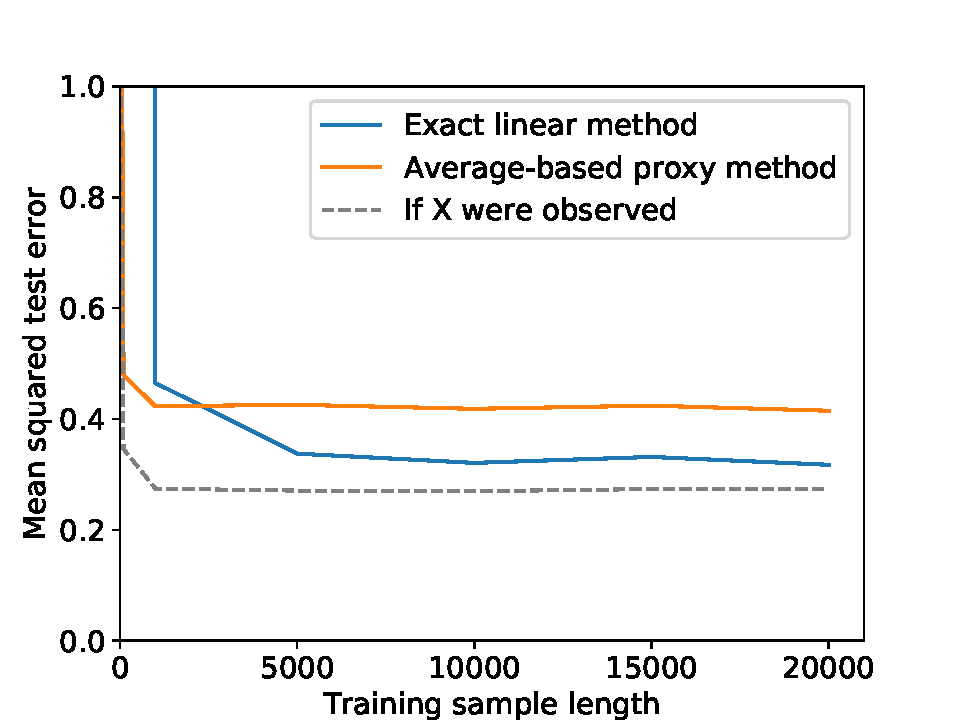
\includegraphics[height=5.8cm]{plotlin} %raw_plots/eval.tex}
	\hspace{-.4cm}
	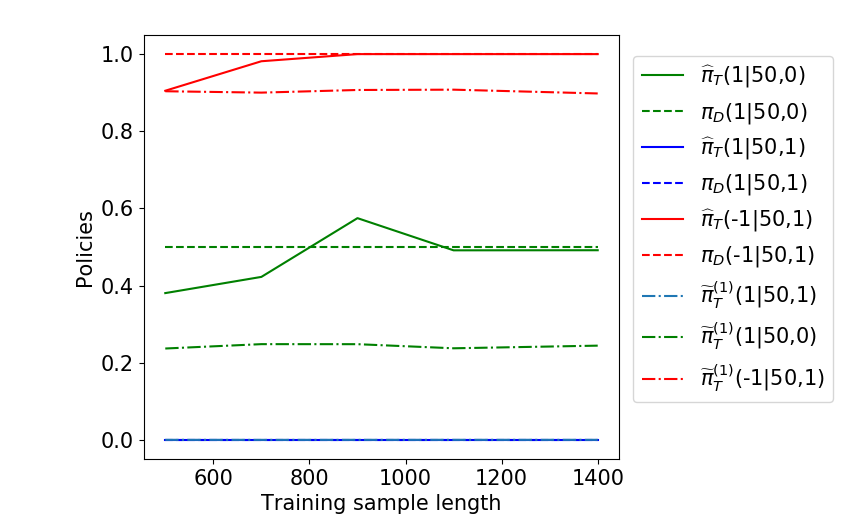
\includegraphics[height=5.5cm]{figure_n.png}
	%%removedVspace
	\caption{\textbf{Left:} Outcome for the action-effect learning experiment. Our exact linear transfer method (Algorithm \ref{alg:lin}) has higher \emph{variance}, but outperforms the average-based proxy method (sample-level version of \eqref{eqn:avp} for linear case), which can be seen as a baseline, for \emph{long enough samples}. We also plot what could be achieved if $X$ was fully observed in the source domain, as a lower bound. \textbf{Right:} Learned policies for the imitation learning experiment: the true policy $\pi_D$, the policy from the method in Section \ref{sec:imex}, $\hat{\pi}_T$, and the corresponding proxy $\tilde{\pi}^{(1)}_T$.
		The three policies are evaluated at three different points $(a|V_o, b_o) \in \{(1|50,0), (1|50,1), (-1|50,1)\}$.}
	\label{fig:explin}
\end{figure*}

\subsection{{Action-effect learning task}}

\paragraph{Setup:}
In this experiment, we test two of our methods for the \dec: Algorithm \ref{alg:lin} and the proxy in \eqref{eqn:avp} (more specifically: a sample-level version of it for the linear case).
We use the real-world data set ``highD'' \cite{highDdataset} that consists of recordings by drones that flew over several highway sections in Germany (mentioned in Example \ref{expl:i}).
From this data set, we selected all situations, where there is a lead car -- the demonstrator (this is a different setup than Example \ref{expl:i}\footnote{While this is the data set mentioned in Example 1, here we do not consider the indicator lights, since for them we would not have the ground truth.}) -- and a following car on the same lane (which are less than 50m from each other, and have speed at least 80km/h).
Here $X$ is distance, velocities, and acceleration of the follower; $A$ is the acceleration of the demonstrator; and $Z$ is the acceleration of the follower, 1.5 seconds later.

Furthermore, the source domain's $Y_S$ is generated by a randomly drawn matrix $F$ applied to $X$ plus Gaussian noise (as in \eqref{eqn:c1}).
This semi-real approach allows us to have ground truth samples from $P(Z, A, X) = P_T(Z, A, Y_T)$, i.e., the target domain (recall our Assumption \ref{asm:d}).
We apply the two methods on training samples from the source domain $P_S(Z, A, Y_S)$ up to length 20000, and calculate the means (over 20 different data and synthetic noise samples) squared error on separate test samples of length 1000 from $P(Z, A, X)$.

\paragraph{Outcome:}
The outcome for this experiment is \emph{depicted and discussed} in Figure \ref{fig:explin}.



\subsection{Imitation learning task}\label{sec:exp_imi}

%\paragraph{Experimental setup:}

\paragraph{Setup:}
In this experiment we simulated the driving scene illustrated in Figure \ref{fig:example1}. The observation set of the demonstrator $\Obs_D$ contains the speed $v_o\in\{40, 45, ...,60\}$ km/h and the indicator light $b_o\in\{0,1\}$ of the lead vehicle. The imitator only gets to see a noisy observation of the demonstrator's speed, i.e., $\Obs_S= v_d + N$, where $N\sim\mathcal{N}(0,1/4)$.  Actions are $-1, +1, 0$ denoting speed reduction by 5km/h, increasing it by 5km/h, and keep the same speed, respectively. In this experiment, we assumed $\Obs_D=\Obs_T$.

We defined the demonstrator's policy to reduce the speed when the indicator of the other vehicle is on $b_o=1$ and increase its speed or keep the same speed when $b_o=0$.
Note that the classical imitation learning approach will fail in this setting since $\Obs_T\neq\Obs_S$.

We applied Algorithm \ref{alg:svd} plus a criterion to obtain the policy $\tilde{\pi}_T^{(1)}$ for the imitator
%\footnote{Codes are available in https://www.dropbox.com/sh/ \\ balilehgpoa18yb/AACEgSRNv1Zv9fZies0b1rj3a?dl=0}.
This criterion (that is described in the supplement) ensures that the imitator neither increases its speed when $b_o=1$ nor decreases its speed with the same probability when $b_o=0$. We formulated this as a linear programming.

\paragraph{Outcome:}

Figure \ref{fig:explin} compares the true policy $\pi_D$, the policy from the method in Section \ref{sec:imex}, $\hat{\pi}_T$, and the corresponding proxy $\tilde{\pi}^{(1)}_T$ for different sample sizes.




\section{Conclusions}
%Sensor-shift is a significant problem in learning from demonstrations, \todo{too strong?} but, so far, barely addressed in a \emph{systematic} fashion. %, rarely addressed practically relevant problem that is barely addressed in a systematic fashionusually not systematically addressed by many classical learning from demonstration methods. %s are a relevant problem are a problem for classical learning from demonstrations

Sensor-shift is a significant problem in learning from demonstrations. In this work, we proposed a principled and general framework to address it, based on causal modeling.
%In this work, we approached it in a principled way using causal models. %f sensor-shift in transfer learning from demonstrations, using causal models. %, %ability of observations of a demonstrator for imitation and in a target domain with different sensors,
We developed novel algorithms that uniquely identify or constrain/approximate the relevant causal effects, and established theoretical guarantees.
The take away message is that the relevant causal relationships may still be identifiable, even if the demonstrator, spectator and target agent have different sensors.


%A surprising insight was that even when our measurements are more noisy than the demonstrator's sensory input, the relevant causal relations may still be identifiable.

%Somewhat su
%We established theoretical guarantees, based on generalizability through modularity.
%We deviced practical algorithms for several sensor-shift scenarios, and validated them in experiments.
%A main insight was that even when our measurements are more noisy than the demonstrator's sensory input, the relevant causal relations can sometimes still be identified.
%Major advantages of our approach are the inspectability, the possibility to give guarantees, and a form of reasoning that enables generalizability through modularity.


Repellendus illum consectetur totam numquam corporis facere ab sequi aliquid, ea dolorem nobis voluptatibus suscipit, incidunt aut labore cumque earum vitae amet reiciendis assumenda et nesciunt, beatae ex velit adipisci placeat quisquam repellat cupiditate totam voluptatem, expedita odio repudiandae?Quisquam earum provident aliquid laboriosam velit error atque ducimus ut cupiditate, similique repellat repellendus tempora beatae error aut blanditiis velit asperiores harum ipsum, nesciunt rem odio incidunt molestiae omnis ullam autem.Earum eligendi illum laboriosam, sint fuga modi enim beatae facilis, cumque fugit recusandae.Accusamus eum maxime placeat labore, praesentium impedit earum obcaecati, perferendis voluptate dolore qui culpa, molestiae voluptatibus sunt nesciunt provident quod nemo magnam fuga totam quasi aspernatur.Quisquam modi veritatis, tempora repudiandae voluptatum.Aliquam laboriosam facilis quas eius odio nam similique, odit dicta illum adipisci ratione perspiciatis provident delectus eveniet, porro facere cumque magnam iusto quaerat vitae deleniti saepe vero veniam?Pariatur delectus doloremque qui optio ex at provident vero dolorem in, necessitatibus odio nemo magni ea reiciendis accusamus laudantium consectetur voluptate eos debitis, necessitatibus fugit distinctio provident nesciunt doloribus odio quam architecto reiciendis esse voluptatum.Vitae debitis perspiciatis commodi, ipsum sapiente repellat consequuntur deserunt ratione corporis temporibus quidem veniam quasi repudiandae?Maxime possimus praesentium doloribus, sit laborum voluptatem labore repellendus qui libero provident, saepe qui exercitationem iure dolores nesciunt optio quas alias nam perferendis, doloribus beatae aperiam modi aliquid eligendi, omnis nisi beatae.Sapiente libero vel eaque architecto magnam provident
\bibliography{causal_traffic}
\bibliographystyle{aaai}
%\bibliographystyle{unsrt}



\end{document}